\subsection{Flöde vid termisk jämvikt}

Vid beräkningen av energiflödet genom grunden användes geometrin som kan ses i figur \ref{fig:groundheat}. Källaren antas vara belägen en halv meter under marknivån.

Som kan ses i figur \ref{fig:cooling_ground} så varierar inte energiflödet mer än en dryg watt per kvadratmeter mellan årstiderna och i många applikationer antas det därför vara konstant. Då vår grund är ungefär $\unit[22]{m}\cdot\unit[13]{m}=\unit[286]{m^2}$ ger detta ett energiutflöde mellan $\unit[3,6]{kW}$ på våren och $\unit[3,2]{kW}$ under tidig höst. 

% Man kan troligen anta att fler människor befinner sig i fastigheten under vintern eftersom det är kallt ute och människor föredrar att vara inomhus i större utsträckning, vilket delvis skulle kunna kompensera för det ökade effektutflödet under den kallare delen av året.

% Således finns det inget behov för att reglera framlednigstemperaturen för energiförluster från grunden. Kan antagas konstant $\approx \unit[3,5]{kW}$. Låter denna siffra rimlig?

\begin{figure}
\centering
\subfloat[Temperaturen i marken den första januari, $^\circ\mbox{C}$.]{
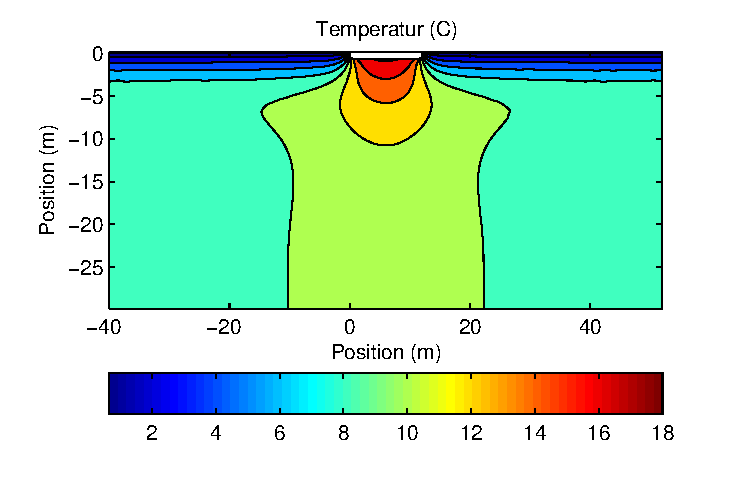
\includegraphics[width=6cm]{images/groundheatdec.eps}
}
\subfloat[Temperaturen i marken den första juli, $^\circ\mbox{C}$.]{
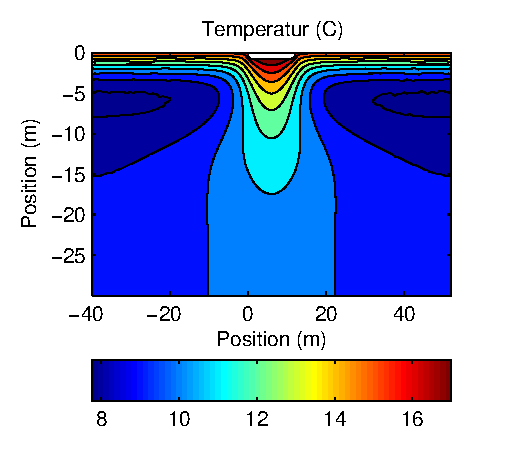
\includegraphics[width=6cm]{images/groundheatjune.eps}
}
\caption{\label{fig:groundheat}
Temperaturen i marken under byggnaden, $\unit{^\circ C}$, beräknat utifrån månadsmedeltemperaturen de senaste 20 åren i Göteborg för två fiktiva dagar i juni respektive januari. Konvektionsparametern är satt till $h=15,5$. }
\end{figure}


\begin{figure}
\centering
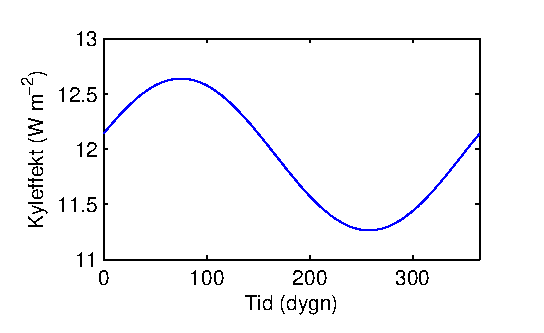
\includegraphics{images/groundcool.eps}
\caption{\label{fig:cooling_ground}
Kyleffekten per kvadratmeter från grunden för medelåret de senaste tjugo åren. Konvektionsparametern är satt till $h=15,5$. }

\end{figure}




